\chapter{\label{chap:chap3}{Research Methodology}}

The main goal of our research is two-folded: to identify a set of criteria suited to evaluate BDD scenarios based on the knowledge of practitioners and to propose a question-based checklist to evaluate BDD scenarios. The output of those questions are meant to help the evaluator decide how good her BDD scenarios are and, if not satisfactory, may be the input of formal or informal scenarios' refinement sessions and other formats of conversations around those scenarios.

\begin{framed}

\indent \textbf{Research Question 1 (RQ1):}

What are the criteria suited to evaluate a good BDD scenario by the view of a software development team member?

\indent \textbf{Research Question 2 (RQ2):}

How does a software development team member evaluates BDD scenarios with those attributes?

\end{framed}

\section{Research Objectives}

This research have the following minor objectives:

\begin{itemize}
    \item \textbf{Objective 1:} To summarize the evaluation characteristics that the written form of BDD scenarios may have, according to the experience of its practitioners;
    \item \textbf{Objective 2:} To summarize the quality attributes applicable to BDD scenarios format;
    \item \textbf{Objective 3:} To link these evaluation characteristics with the quality attributes applicable to BDD scenarios format;
    \item \textbf{Objective 4:} To propose a question-based-checklist, that would guide the reader during the quality evaluation of BDD scenarios.
\end{itemize}

\section{Research Design}

Since there is no standard on what is considered a ``good'' scenario due to the few views on this matter, this is a concept that still needs to be fully understood. A qualitative approach is suitable for situations like this \cite{Creswell_2008}. Also, we believe the opinions from industry practitioners working on multiple companies and contexts would be a natural input to construct a quality concept for BDD scenarios. Therefore, we judge that the use of an empirical approach would suit our research goal and questions. Finally, we decided to collect data using semi-structured interviews, as we value multiple different opinions taken from different contexts.

To achieve our research goal, we proposed a multiple-steps research design as presented in Figure \ref{fig:research_design}, where the light gray boxes are the studies/actions that achieved the outputs shown in the dark gray boxes. This design was based upon the understanding that interviews with open-ended questions alone would not provide enough data to formulate a proper question-based checklist due to the participants' plurality of terms and opinions. Therefore, we judged necessary to have our interviews guided by a set of quality attributes that had previously been used to evaluate BDD scenarios.

First, we had to discover what are those literature quality criteria. A literature review (Figure \ref{fig:research_design}, Study A) has confirmed that traditional attributes \cite{Babok_2009}\cite{Babok_2015} and the INVEST\cite{Cohn_2004} acronym were used with agile requirements. That literature review was reported as a technical report \cite{Literature_Review_Technical_Report_2018}.

Additionally, we acquired some knowledge about how evaluators judge the quality of BDD scenarios using those attributes. To that end, we conducted a pilot study (Figure \ref{fig:research_design}, Study B) with 15 graduate students to understand how they evaluate BDD scenarios. The output of this pilot study was the sub-set of literature attributes that were used to guide the debate with practitioners -- shown as Output 2 in Figure \ref{fig:research_design} and reported in the 2017 Workshop on Empirical Requirements Engineering (EmpiRE'17) in conjunction with the International Requirements Engineering Conference \cite{Empire_2017}.

\begin{figure}[t]
\centering
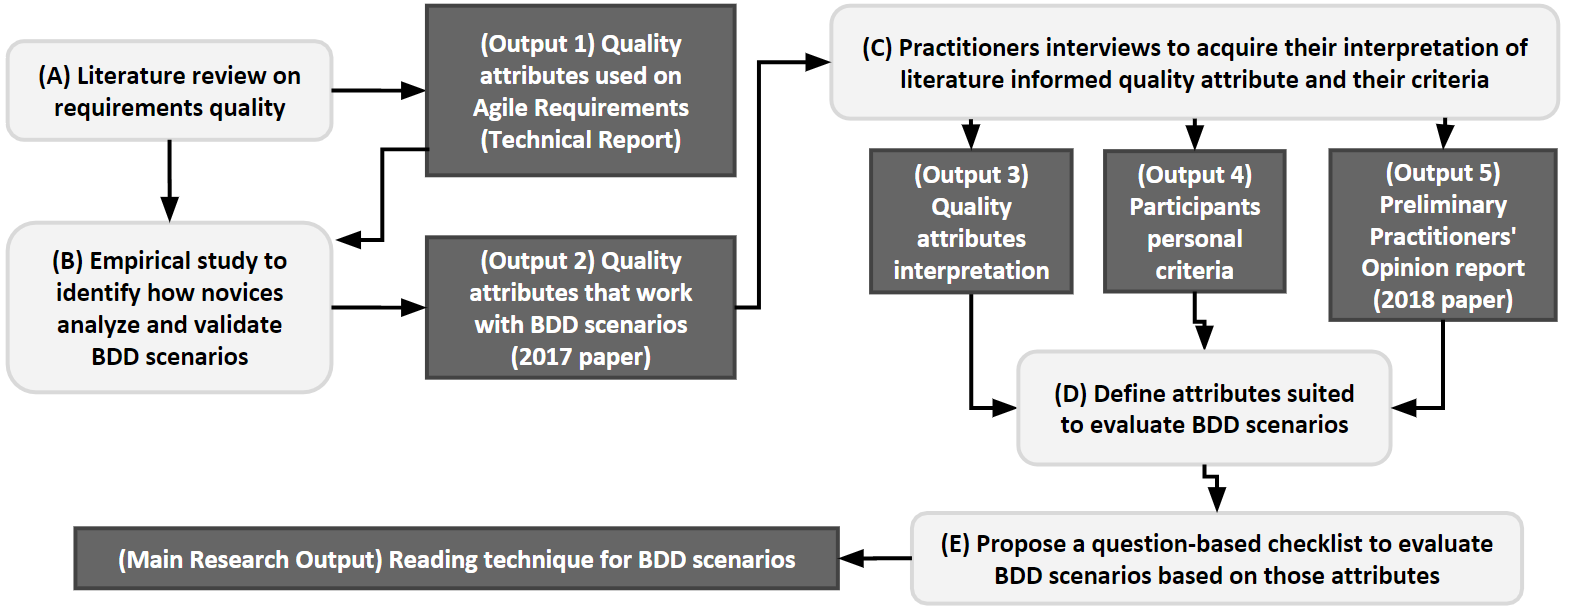
\includegraphics[width=.9\textwidth]{images/Research_Plan}
\caption{Research Design}
\label{fig:research_design}
\end{figure}

In addition to those literature quality attributes, we used real-life examples of BDD scenarios during our interviews to aid practitioners realize their own quality criteria. To avoid our own bias towards what would be a good or bad BDD scenario, we decided to not create the examples ourselves. Instead, we handed them real BDD scenarios, taken from an open source project that employ BDD scenarios to detail their applications' behavior. 

To find those real BDD scenarios, we searched Github's\footnote{\url{https://github.com/}} repository database. Due to the fact that BDD scenarios are automated, they are often carried along with the application source code as the tests to that system. Due to the popularization of tools like Cucumber \cite{Wynne_and_Hellesoy_2012}, BDD's feature files are saved with the extension ``.gherkin''. Github's search feature allowed us to filter repositories by the types of files they used, an advanced functionality missing in other known repositories of source code. Therefore, we filtered our search for the gherkin extension. That search resulted in Diaspora\footnote{\url{https://diasporafoundation.org/}}, a decentralized social network with a list of feature files mapping the behavior of the different application screens. To the best of our knowledge, Diaspora is Github's open source project with the most feature files available.

Besides the literature-informed quality attributes and the real-world example of BDD scenarios, we sometimes provoked participant's thoughts using a list of experience-based criteria taken from Smart's book \cite{Smart_2014} and Wynne and Hellesoy's book \cite{Wynne_and_Hellesoy_2012}, such as: steps too long/too short; too few/many steps; business language usage; title description; keywords (Given/When/Then) usage and order; repetition of steps. That list was kept hidden from the participant's -- certain items were used whenever we judged necessary, as additional questions to refine their analysis of Diaspora's scenarios.

Our semi-structured interviews (Figure \ref{fig:research_design}, Study C) produced practitioners' interpretations of literature-informed quality attributes (Output 3, reported in Section \ref{chap:chap4_attributes}) and their own personal evaluation criteria (Output 4, reported in Section \ref{chap:chap4_criteria}). With that data at hand, we were able to define quality attributes to suited to evaluate BDD scenarios (Action D, reported in Section \ref{chap:chap4_analysis}) and answer our RQ1. Composing those newly-defined attributes into a question-based checklist (Action E, reported in Chapter \ref{chap:chap5}), similar to the questionnaire Cockburn \cite{Cockburn_2000} uses for Use Cases, we reached the answer to our RQ2. A preliminary report of our semi-structured interview (with 8 practitioners) results is reported in the 2018 International Working Conference on Requirements Engineering (REFSQ'18) paper \cite{Refsq_2018}. 

Action D's initial purpose was to refine the sub-set of literature-informed quality attributes. However, as we could not decide for ourselves what interpretation of each attribute is more suited than others without enforcing our own bias, we used them all as characteristics, regardless of what literature attribute generated it, and composes them into newly-labeled quality attributes.

\subsection{Pilot Study}

Our pilot study (Figure \ref{fig:research_design}, Study B) aimed to provide us some knowledge about how evaluators judge the quality of BDD scenarios using quality attributes found on the literature review (Figure \ref{fig:research_design}, Study A). Therefore, we organized a study with 15 graduate students, all with previous industry experience as developers, technical leads, or managers. They also have declared to know well how to write use cases, and to a lesser extent how to write user stories or BDD scenarios. The literature quality attributes used were: atomic, complete, consistent, concise, estimable, feasible, independent, negotiable, prioritized, small, testable, understandable, unambiguous, and valuable.

During the study, the students were first asked to write requirements for two fictional products (PA and PB) in two different formats -- use cases (UC) and user stories with BDD scenarios (US+BDD). Later, each student evaluated the work of 2 others colleagues using the literature quality attributes we have listed before. This cross-activity design exemplified in Table \ref{table:study_organization} helped us reduce the risk of the evaluator lacking understanding of the application domain under analyses and of the evaluator's reading ability being driven by the same writer's bias.

\begin{table}[t]
	\renewcommand{\arraystretch}{1}
	\caption[Cross-activity design of pilot study]{Cross-activity design of pilot study. Source: \cite{Empire_2017}}
	\label{table:study_organization}
	\centering
	\begin{tabular}{|m{1cm}|m{3cm}|m{3cm}|m{3cm}|m{3cm}|}
		\hline
		\textbf{ID} & \textbf{Task 1} & \textbf{Task 2} & \textbf{Task 3} & \textbf{Task 4}\\
		\hline
		S1 & Write UC\newline for PA & Write\newline US+BDD\newline for PB & Evaluate\newline US+BDD\newline for PA\newline\textit{(S2 task 1)} & Evaluate\newline UC\newline for PB\newline\textit{(S4 task 2)}\\
		\hline
		S2 & Write\newline US+BDD\newline for PA & Write\newline UC\newline for PB & Evaluate\newline UC\newline for PA\newline\textit{(S1 task 1)} & Evaluate\newline US+BDD\newline for PB\newline\textit{(S3 task 2)}\\
		\hline
		S3 & Write\newline UC\newline for PA & Write\newline US+BDD\newline for PB & Evaluate\newline US+BDD\newline for PA\newline\textit{(S4 task 1)} & Evaluate\newline US+BDD\newline for PB\newline\textit{(S2 task 2)}\\
		\hline
		S4 & Write\newline US+BDD\newline for PA & Write\newline UC\newline for PB & Evaluate\newline UC\newline for PA\newline\textit{(S3 task 1)} & Evaluate\newline US+BDD\newline for PB\newline\textit{(S1 task 2)}\\
		\hline
	\end{tabular}
\end{table}

From this pilot study, we have acquired the literature quality attributes that could potentially work with BDD scenarios, according to the opinion of the novice BDD evaluators, students with industry experience. Therefore, the literature-informed quality attributes used later in the semi-structured interviews are: concise, estimable, feasible, negotiable, prioritized, small, testable, understandable, unambiguous, and valuable. 

\subsection{Interview's Participants Selection}

In order to identify the first participants for our interviews, we organized a survey to both acquire a grasp of people's opinion about BDD quality topic and their contact information. The survey, titled as \textit{Do you believe BDD scenarios' quality matter?}, posed two statements and an entry to collect a respondent's contact information for later follow up. Answers to the statements ranged from 1 (Totally Disagree) to 5 (Totally Agree). The statements were:

\begin{enumerate}
    \item Well written BDD scenarios directly impacts the final product quality.
    \item It is important to have a standard set of criteria to evaluate written BDD scenarios' quality.
\end{enumerate}

The survey was shared on the social network (such as Twitter\footnote{\url{https://www.twitter.com}} and Linkedin\footnote{\url{https://www.linkedin.com}}) profiles of the thesis author and on BDD virtual communities such as Cucumber slack channel\footnote{\url{https://cucumberbdd.slack.com/messages/C590XDQQH/}}, BDD London slack Channel\footnote{\url{https://bddlondon.slack.com/messages/C1BMRM2HX/details/}}, Ministry of Testing forum\footnote{\url{https://club.ministryoftesting.com/t/do-you-believe-bdd-scenarios-quality-matter/1449}} and slack channel\footnote{\url{https://ministryoftesting.slack.com/messages/C0RUQE6V8/}}. 
We got 99 answers to the survey, detailed in Figure \ref{fig:survey_answers}, with the large majority of the respondents agreeing with the previously presented statements. However, contrary to our beliefs, the follow up e-mails inviting people to a larger interview session were not answered accordingly.  

\begin{figure}[t]
\centering
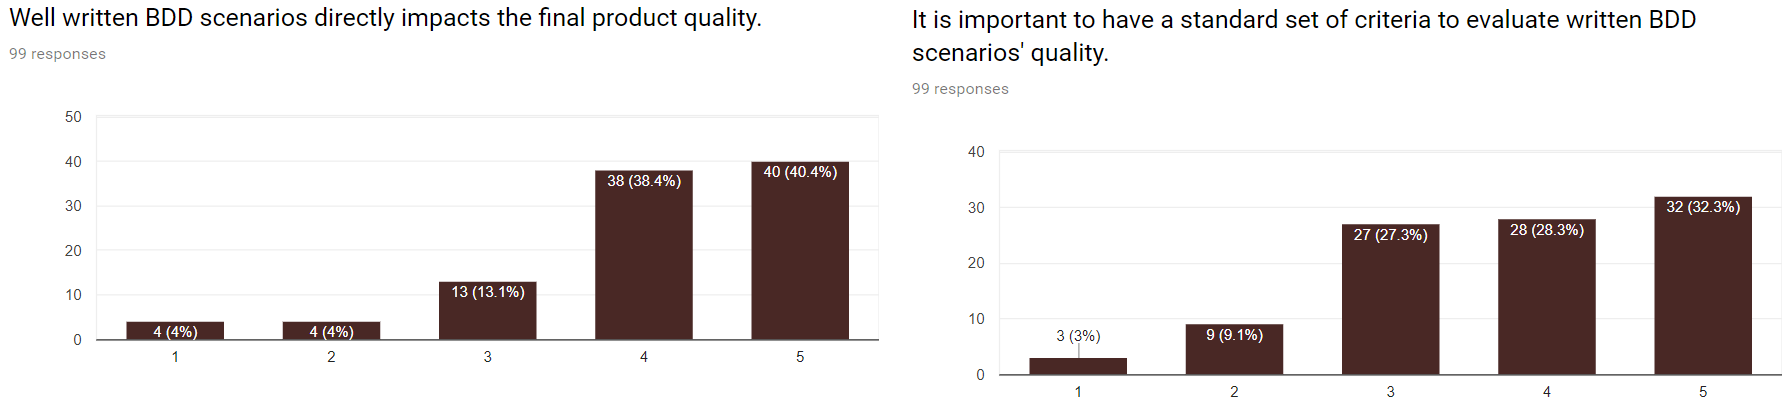
\includegraphics[width=.9\textwidth]{images/survey_answers}
\caption{Survey Answers' Statistics}
\label{fig:survey_answers}
\end{figure}

Therefore, we changed our focus to direct searches on this thesis' author Linkedin social-network. Our belief was that a more personal touch, showing the author's profile (someone who works in industry with test automation and has experience with BDD for over 5 years) to potential participants, would improve our chances. The search feature on the website\footnote{\url{https://www.linkedin.com/help/linkedin/answer/302/searching-on-linkedin}} was heavily used, returning data from the inside of the thesis' author network but also from the outside -- up to 3 connections of distance. Using the terms ``BDD'' and ``Behavior-Drive-Development'', every search returned experienced BDD practitioners. Within every practitioner profile, we double-checked the existence of BDD experience and proceeded to invite the person to connect and dedicate their time in an 1hr slot interview. By the time of the writing of this thesis, 79 invitations were accepted and 34 invitations were not answered. From those who accepted to connect, only 18 accepted to participate in the interviews. All those 18 participants' profiles are reported in Section \ref{chap:chap4_profile}.

\subsection{Interview Design}

Taking inspiration on the questions used by Heck and Zaidman \cite{Heck_and_Zaidman_2017} on their interviews with practitioners to understand how user stories' quality can be understood, we list in Table \ref{tbl:questions} the set of questions to capture practitioners views and opinions on our interviews, to disclose how they use BDD scenarios to perform their tasks during a software development cycle, and to identify how they evaluate if those scenarios are ready to be used. 

The authors' original interview script \cite{Heck_and_Zaidman_2017} was organized into two parts -- one performed with minimal introduction from their side and without showing the participants their framework and another in which they asked the participants to use their framework, transformed into a checklist, on some examples taken from open source projects. 

\begin{table}[t]
	\caption{Interview Questions}
	\label{tbl:questions}
	\centering
	\begin{tabular}{|m{0.5cm}|m{12cm}|}
		\hline
		\multicolumn{1}{|c|}{\textbf{ID}} & \multicolumn{1}{|c|}{\textbf{Question}}\\
		\hline
		1 & What is your role on the project?\\
		\hline
		2 & What is your main task on the project?\\
		\hline
		3 & For how long do you use BDD?\\
		\hline
		4 & How does your project use BDD scenarios?\\
		\hline
		5 & What do you pay attention to when evaluating BDD scenarios?\\
		\hline
		6 & On Diaspora, evaluate a feature file according to your criteria.\\
		\hline
		7 & Do quality attributes help evaluating BDD scenarios?\\
		\hline
		8 & What is the meaning of each attribute on BDD scenarios?\\
		\hline
		9 & On Diaspora, evaluate a feature file according to the attributes.\\
		\hline
		10 & Do you miss any other attribute?\\
		\hline
		11 & What quality attributes did you find difficult to use?\\
		\hline
		12 & To what extent the attributes helped you evaluate a scenario?\\
		\hline
		13 & How your criteria maps to those attributes?\\
		\hline
	\end{tabular}
\end{table}

In a similar way, the open ended questions in our interview script in Table \ref{tbl:questions} were crafted to acquire the participants views before presenting their own and help us answer our \textbf{RQ1}, while the act of actively using literature-informed quality attributes to evaluate Diaspora's examples aid on our \textbf{RQ2}. The four starting questions were used to understand the participants' profile and their answers are presented in Section \ref{chap:chap4_profile}. 

Questions 6 and 9 asked the participant to actively use examples of BDD scenarios taken from Diaspora project and evaluate them, either with their own personal criteria or the literature-informed quality attributes. From the 47 feature files available to cover Diaspora's desktop version, the participants were asked to choose one to evaluate as part of question 6 and another, different one, to evaluate as part of question 9. The interviewer did not influenced their decision in any way. 

Questions 5 and 6 were useful to acquire participant's criteria without any bias of our list of literature-based quality attributes and their answers are reported in Section \ref{chap:chap4_criteria}. If only a few answers emerged for those questions, we provoked their thoughts using the experience-based criteria from Smart \cite{Smart_2014} and Wynne and Hellesoy \cite{Wynne_and_Hellesoy_2012} books, as explained in the Chapter \ref{chap:chap2_agile_quality}.

Questions 7 to 11 were useful to acquire participant's interpretations of our literature-informed quality attributes and are analyzed in Section \ref{chap:chap4_attributes}. 

Taking the RQs lens, Questions 5 and 8 helped reveal the meaning practitioners see on quality attributes and on their own criteria, thus allowing the newly defined quality attributes that answer our RQ1 to emerge. In addition, Questions 6 and 9 gave us insights on how those attributes and personal criteria were used in practice, providing important information to answer RQ2 and define our question-based checklist. 

Question 12 was useful to assess how useful such a list was and tease the interviewee to suggest better ways to evaluate BDD scenarios. Question 13 asks the participant to link those literature quality attributes with their own criteria, tying those attributes with practical details of BDD scenarios and motivating us to threat interpretations and criteria altogether in our checklist. That question was a final check in case the conversation have not linked participant's criteria and interpretations to attributes. Our initial thought was that this mapping would be useful to join good and bad practices, that emerged from practitioner's personal criteria, with literature-based quality attributes. However, this intention was not successful, due to the different interpretations of each attribute. As explained before, we decided to use all interpretation of each literature-based attribute as characteristics to avoid choosing which of those interpretations was best suited for each literature quality attribute. Additionally, the participants' personal evaluation criteria were also treated as characteristics. Those characteristics were later grouped together into newly-redefined quality attributes, that compose our proposed question-based checklist as presented in the following sections.

Before starting those interviews, the script was validated by a doctoral student with 4 years of previous experience in industry. Additionally, a pilot interview was conducted with a software tester who has about 6 years of experience with BDD usage. He reinforced our idea of using Smart's \cite{Smart_2014} and Wynne and Hellesoy's \cite{Wynne_and_Hellesoy_2012} experience-based criteria to provoke the discussions in Questions 5 and 6 from Table \ref{tbl:questions}. 

\subsection{Data Analysis}

In total, we interviewed 18 practitioners. Each interview lasted in average 77 minutes, being the longest 1 hour and 51 minutes and the shortest 62 minutes long -- a total of 1390 minutes were recorded. The interviews were conducted via Skype\footnote{\url{https://www.skype.com}} tool and were voice-recorded (with documented permission). The interviews were performed either in English or Portuguese during a period of 3 months (from September to November in 2017) and then manually transcribed to the participant’s native language. The quotes were translated to English whenever a certain reference to it was needed. We realized we had reached saturation when no new practitioner quality criteria was found. That is when we decided to stop the interview process and start the findings compilation.

\begin{figure}[t]
\centering
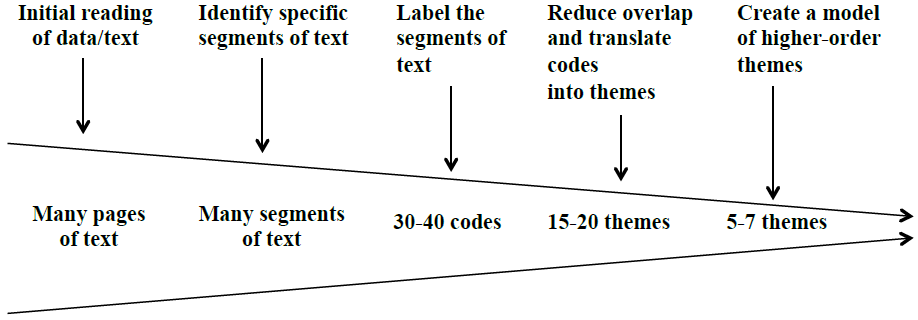
\includegraphics[width=.9\textwidth]{images/thematic_synthesis}
\caption{Thematic synthesis process. Source \cite{2011_Cruzes_and_Dyba}}
\label{fig:thematic_synthesis}
\end{figure}

Cruzes and Dyba state \cite{2011_Cruzes_and_Dyba} that a number of different methods have been proposed for the synthesis of qualitative and mixed-methods findings such as the ones we typically find in software engineering (SE), which lead them to conceptualize thematic synthesis in SE. Thematic synthesis, whose process is presented in Figure \ref{fig:thematic_synthesis}, draws on the principles of thematic analysis and other established methods in primary qualitative research to identify the recurring themes or issues in the primary sources of data, analyzes these themes, and draws conclusions from them. 

Coding is a method that enables the researcher to organize and group similar data into categories because they share some characteristic -- the beginning of themes \cite{2011_Cruzes_and_Dyba}. All our text was coded in English, even tough our interviews' data were both in English and Portuguese -- a process made possible by the fact that both the main researcher, who interviewed the participants and coded the data, and the advisor, who reviewed the codes, reads and speaks both languages. Coding can be performed using one of the following approaches:

\begin{enumerate}
    \item \textbf{Deductive approach:} starting with a start list of preconceived codes, data is analyzed and coded accordingly. Cruzes and Dyba \cite{2011_Cruzes_and_Dyba} state that great care must be taken to avoid forcing data into these categories because a code exists for them;
    \item \textbf{Inductive approach:} Cruzes and Dyba \cite{2011_Cruzes_and_Dyba} state that the inductive approach reviews data  line by line in detail and, as a concept becomes apparent, a code is assigned. Upon further review of data, the analyst continues to assign codes that reflect the emerging concepts, highlighting and coding lines, paragraphs, or segments that illustrate the chosen concept;
    \item \textbf{Integrated approach:} the integrated approach is meant to mix both the deductive and the inductive approach, creating a general accounting scheme for codes that is not content specific, but points to general domains in which codes can be developed inductively \cite{2011_Cruzes_and_Dyba}.
\end{enumerate}

Knowing that we specifically decided to guide our interviews with literature-informed quality attributes (Questions 7 to 11 from Table \ref{tbl:questions}) and with author's experience-based criteria \cite{Smart_2014}\cite{Wynne_and_Hellesoy_2012} (Questions 5 and 6 from Table \ref{tbl:questions}), we used those as initial thematic analysis codes only, taking a integrated approach and assuming they would be refined along with the interviews responses.

\begin{figure}[t]
\centering
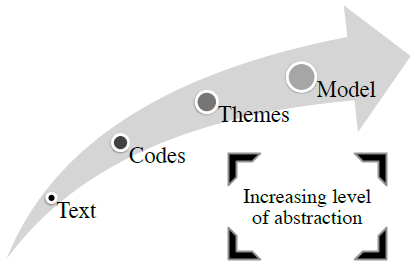
\includegraphics[width=.6\textwidth]{images/thematic_synthesis_abstractions}
\caption{Levels of interpretation in thematic synthesis. Source \cite{2011_Cruzes_and_Dyba}}
\label{fig:thematic_synthesis_abstractions}
\end{figure}

Themes are the outcome of coding, categorization, and analytic reflection, but also a way of grouping the initial codes into a smaller number of sets \cite{2011_Cruzes_and_Dyba}. We refined the initial thematic analysis codes into themes during our cyclical analysis, resulting in the newly-redefined quality attributes (Action D from Figure \ref{fig:research_design}, reported in Section \ref{chap:chap4_analysis}) that composes our proposed question-based checklist (Action E from Figure \ref{fig:research_design}, reported in Chapter \ref{chap:chap5})

The connection between these different levels of abstractions, from codes (literature-informed quality attributes and author's experience-based criteria) to themes (the newly-defined quality attributes) until a model is formed (the proposed question-based checklist), can be seen in Figure \ref{fig:thematic_synthesis_abstractions}. Codes were grouped together in a mind map, constructed in the XMind\footnote{\url{www.xmind.net/}} software. The mapping between our codes and themes is found in Table \ref{tbl:characteristics_mapping}, where the characteristics (codes) are mapped to themes (newly-defined attributes).

\subsection{Threats to Validity}

The fact that only the author of this thesis was involved into the coding process may have impacted the themes creation in an unforeseen way, even with the careful review of the advisor. 

Additionally, we have not taken into consideration the gender, role, location nor the type of industry a participant works into to reflect upon the data taken from the interviews. We understand that different life experiences may have brought different quality criteria and opinions, so we tried to mitigate this effect interviewing people from many different areas and companies. 

The choice of using BDD scenarios from the Diaspora open source real-life project might also be a threat to the interview results. Choosing different sets of BDD scenarios might have yield different results than ours. We discussed this matter during the interview validation and pilot interview, and both professionals judged Diaspora's feature files as good representatives of real world BDD scenarios. 

Finally, we could have phrased the items in our question-based checklist in many different ways, so we have to acknowledge that our own language bias may have driven us to write them in that way presented in Chapter \ref{chap:chap5}. A specialist review of that question-based checklist is listed as a future work to avoid this threat.